\documentclass[12pt]{beamer}
\usepackage[T1]{fontenc}
\usepackage[utf8]{inputenc}
\usepackage[brazil]{babel}
\usepackage{graphicx}
\usepackage{alltt}
\usepackage{xcolor}

\graphicspath{ {./images/} }
\usetheme{Antibes}
\usecolortheme{default}

\usepackage{amssymb,amsmath}
\usepackage{textgreek}
\usepackage{tikz}

%\hypersetup {
%  pdftitle = {?},
%  pdfauthor = {?},
%  pdfsubject = {?},
%  pdfkeywords = {?}
%}

\setbeamertemplate{headline}{}
\setbeamertemplate{navigation symbols}{}

\title{Interações entre Droga e Doença por meio de Genes}
\author{
  Mateus Siqueira Batista\and
  Nicolas Bissoli Nattis
}
\institute{
  MC536 - Instituto de Computação, UNICAMP
}
\date[2020]{2020}

\begin{document}

\frame{\titlepage}

\begin{frame}
  \frametitle{Proposta}
  Obter dados de interações entre genes e drogas, e entre genes e doenças.
  \pause

  Através disso, podemos relacionar a interação entre estas drogas e as doenças.
  \pause

  \begin{block}{Exemplo:}
    \begin{itemize}
      \item Droga A ativa o gene X.
      \item Gene X tem relação de causa com as doenças \textalpha, \textgamma.
      \item Portanto, a droga A tem relação de causa com as doenças \textalpha, \textgamma.
    \end{itemize}
  \end{block}
\end{frame}

\begin{frame}
  \frametitle{DGIdb}
  \centering
  
\includegraphics[scale=0.5]{dgi}
  \vspace*{1 cm}
  \begin{itemize}
    \item Dados sobre interações droga-gene e o genoma drogável.
    \item Extraído de mais de trinta fontes confiáveis.
    \item Dados extraídos via arquivo .tsv disponibiliszados.
  \end{itemize}
\end{frame}

\begin{frame}
  \frametitle{DisGeNet}
  \centering
  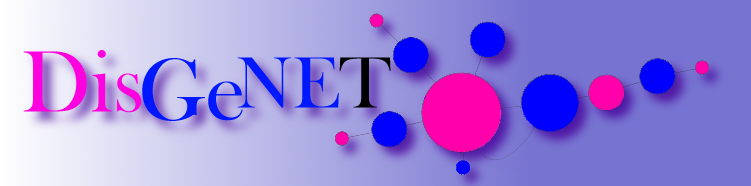
\includegraphics[scale=0.25]{disgenet}
  \vspace*{1 cm}
  \begin{itemize}
    \item Plataforma contendo uma das maiores coleções publicamente disponíveis
          de genes e variantes associados a doenças humanas.
    \item Dados extraídos via banco de dados SQLite disponibilizado.
  \end{itemize}
\end{frame}

\begin{frame}[fragile]
  \frametitle{Lógica}

  A relação de droga-doença ocorre de modo intuitivo a partir das relações de
  doença e droga com o gene.

  \vspace*{0.1cm}

  \begin{tabular}{| c c | c c |}
    \hline
    & & \multicolumn{2}{c|}{Droga-Gene} \\
    & & ativação & inibição \\
    \hline
    Gene-Doença & ativação & ativação & inibição \\
    & inibição & inibição & ativação \\
    \hline
  \end{tabular}

\end{frame}

\begin{frame}[fragile]
  \frametitle{Tipos de Interação}

  \centering
  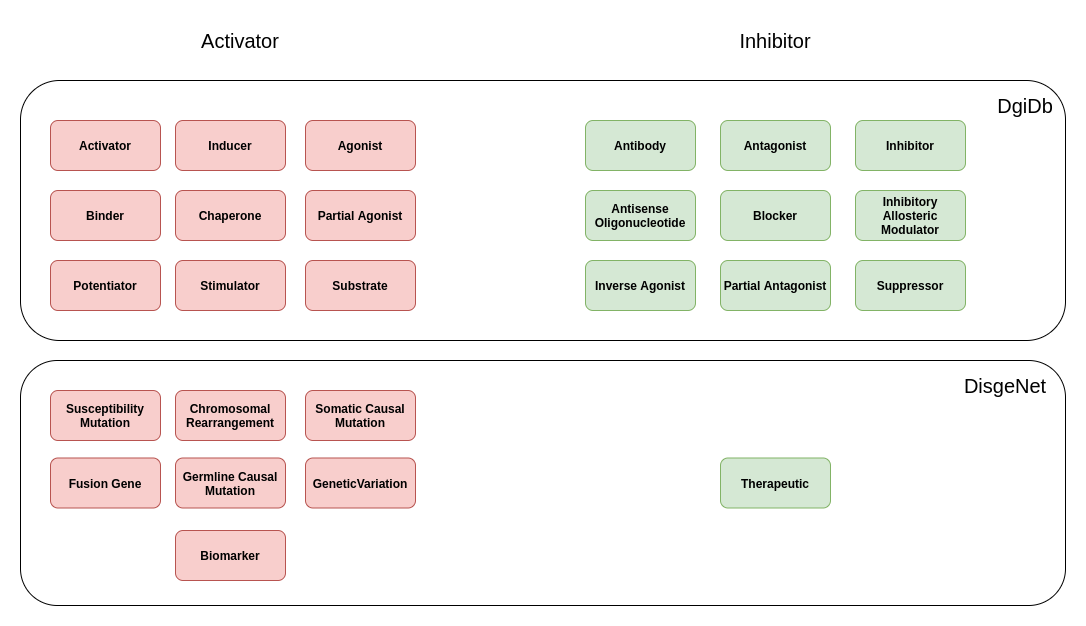
\includegraphics[scale=0.29]{diagram.png}
\end{frame}



\begin{frame}[fragile]
  \frametitle{Modelo Conceitual}
  \centering
  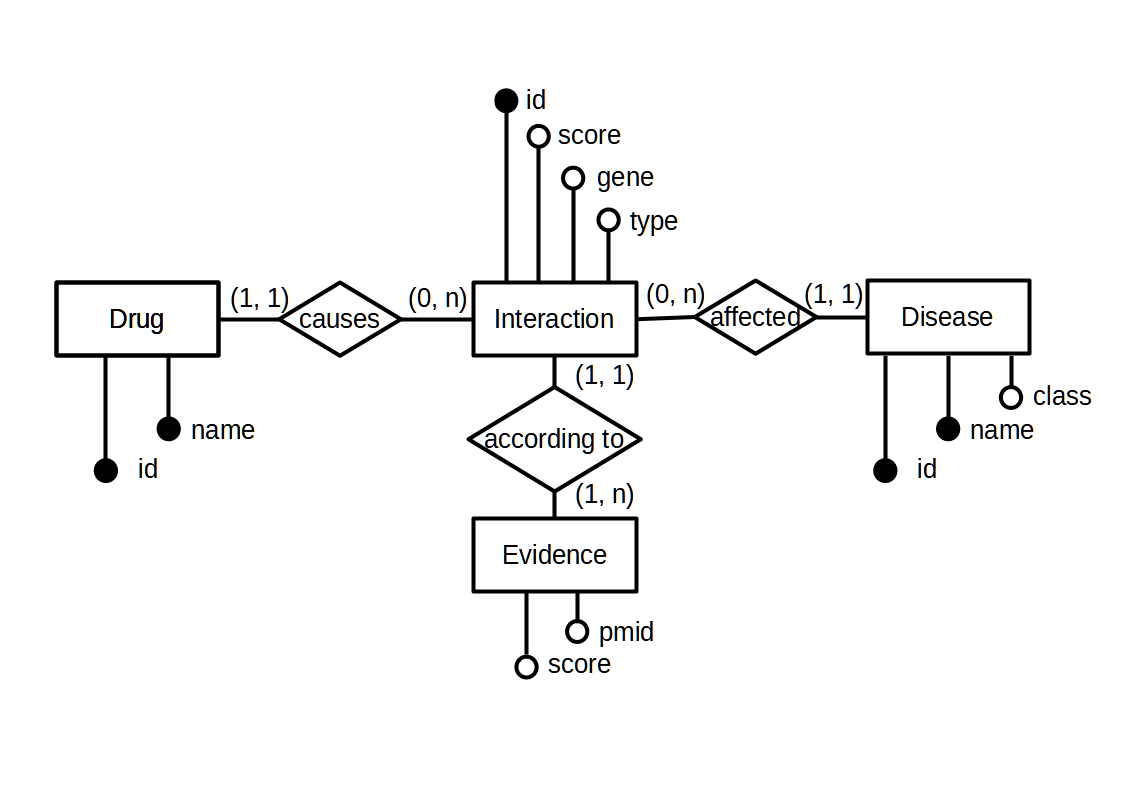
\includegraphics[scale=0.275]{conceitual.png}
\end{frame}

\begin{frame}[fragile]
  \frametitle{Modelo Lógico}

  \begin{alltt}
    Drug(\textcolor{blue}{\underline{DrugId}}, \underline{Name})
    
    Disease(\textcolor{red}{\underline{DiseaseId}}, \underline{Name}, Class)
    
  \end{alltt}
\end{frame}

\begin{frame}[fragile]
  \frametitle{Modelo Lógico}

  \begin{alltt}
    Interaction(\underline{InteractionId},
                \textcolor{blue}{DrugId},
                \textcolor{red}{DiseaseId},
                Score,
                Gene,
                Type)
               
    Evidence(\textcolor{teal}{InteractionId},
                Pmid,
                Score)
                  
  \end{alltt}
\end{frame}

\begin{frame}[fragile]
  \frametitle{Modelo Lógico de Redes Complexas}
  \centering
  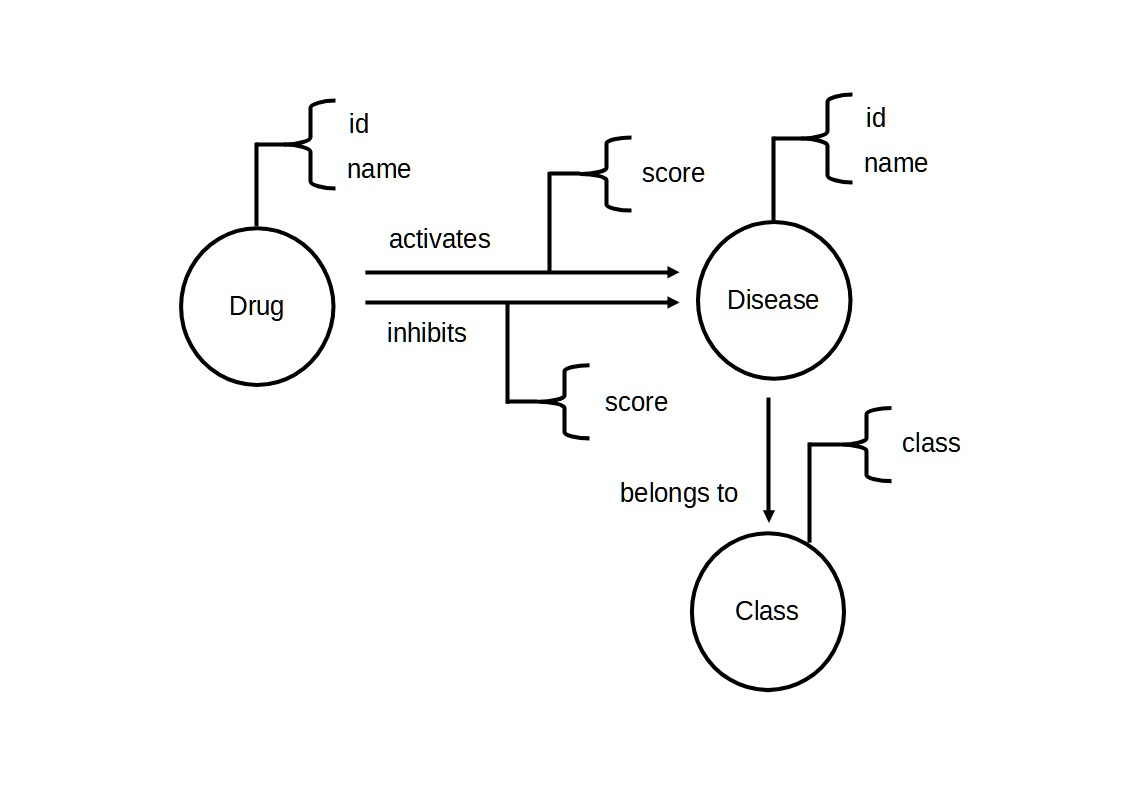
\includegraphics[scale=0.275]{grafo.png}
\end{frame}

\begin{frame}[fragile]
  \frametitle{Evolução do projeto}
  
  \begin{itemize}
    \item Removemos classes de drogas e aliases (fora do escopo).
    \item Dividimos as interações do Neo4j em duas.
    \item Usamos SQLite e TSV ao invés de requisições HTTP (muito lento).
  \end{itemize}
\end{frame}

\begin{frame}[fragile]
  \frametitle{Transformação}

  \begin{itemize}
    \item Transformar DISGENET SQLite em TSV.
    \item Ler TSV das fontes.
    \item Produzir TSV final.
    \item Transformar TSV final em SQLite.
    \item Transformar TSV final em CSV para Neo4j.
  \end{itemize}
\end{frame}

\begin{frame}
  \frametitle{Tratamento de Dados}

  \begin{itemize}
    \item Confibialidade
          \begin{itemize}
            \item Os dados coletados possuem níveis de confiabilidade
                  variáveis, que foram levados em conta e tranformados em um \underline{Score}.
            \item Há um Score atrelado ao \textcolor{blue}{DgIdb} e outro ao \textcolor{red}{DisGeNET}. Assim, obtivemos um Score global da interação multiplicando um pelo outro.      
          \end{itemize}
  \end{itemize}
\end{frame}

\begin{frame}
  \frametitle{Dados publicados}

  \centering
  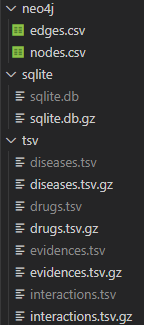
\includegraphics[scale=0.7]{ls}
\end{frame}

\begin{frame}
  \frametitle{Perguntas de Análise}

  Selecione o nome das drogas e doenças das N interações com maior pontuação.

  \only<1>{
  \begin{alltt}\small
SELECT Dr.Name, Di.Name, I.Type, I.Score

FROM Interaction as I, Drug as Dr, Disease  as Di

WHERE Dr.Id = I.DrugId AND Di.Id = I.DiseaseId

ORDER BY I.Score DESC LIMIT 10;
  \end{alltt}
  }

  \only<2>{
    \centering
    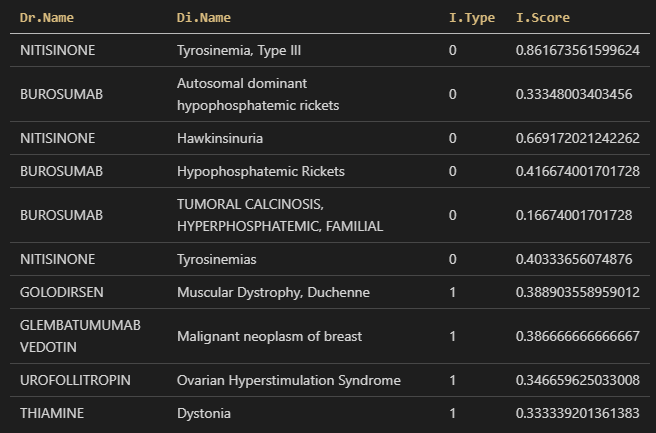
\includegraphics[scale=0.5]{q1}
  }

\end{frame}

\begin{frame}
  \frametitle{Perguntas de Análise}

  Quais drogas tem relação com a doença (Acute lymphocytic leukemia) C0023449?

  \only<1>{
  \begin{alltt}\small
SELECT Dr.Id, Dr.Name, I.Type, I.Score

FROM INTERACTION as I, DRUG as Dr, Disease as Di

WHERE Di.id ='C0023449' AND I.DiseaseId = Di.id

ORDER BY I.Score DESC LIMIT 10;
  \end{alltt}
  }

  \only<2>{
    \centering
    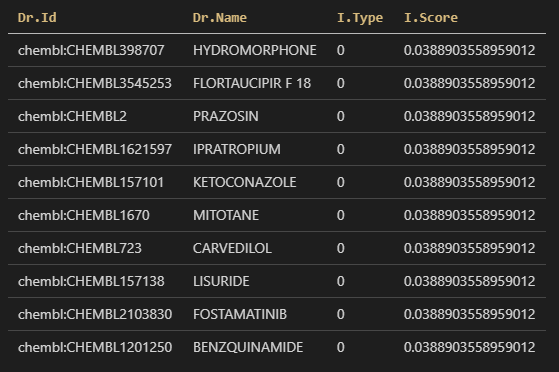
\includegraphics[scale=0.5]{q2}
  }

\end{frame}

\begin{frame}
  \frametitle{Perguntas de Análise}

Quais classes de doenças são mais ativadas pela HYDROMORPHONE?

\only<1>{
  
  \begin{itemize}
    \item Uma análise aprofundada é necessária, mas podemos partir da
          seguinte.
  \end{itemize}

  \begin{alltt}\small
MATCH (dr:Drug)-[activates]->(di:Disease)

-[belongs]->(c:Class)

WHERE dr.name='HYDROMORPHONE'

RETURN dr, activates, di, belongs, c
  \end{alltt}
  }

  \only<2>{
    \centering
    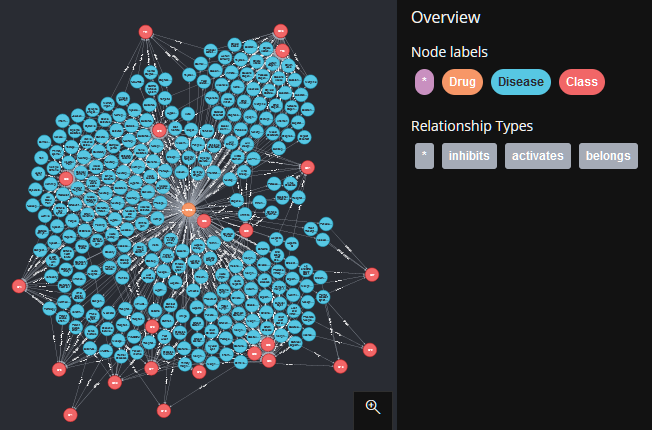
\includegraphics[scale=0.5]{grafo1}
  }

\end{frame}

\begin{frame}
  \frametitle{Perguntas de Análise}

  \begin{itemize}
    \item Podemos deduzir novas interações a partir do grafo?
    \begin{itemize}
      \item Predição de links.
    \end{itemize}

    \item Existem tipos de drogas e doenças que interagem mais entre si?
    \begin{itemize}
      \item Comunidade.
    \end{itemize}
  \end{itemize}

\end{frame}

\begin{frame}
  \centering Obrigado pela atenção!
\end{frame}

\end{document}
